\documentclass[a4paper,14pt]{article}

% Поддержка русского языка
\usepackage[T1, T2A]{fontenc}    % Кодировка
\usepackage[utf8]{inputenc}  % Кодировка исходного текста
\usepackage[english, russian]{babel}  % Локализация и переносы
\usepackage{titlesec, titletoc} % Для настройки стилей заголовков и содержания
\usepackage{booktabs} % Для использования \toprule, \midrule и \bottomrule
\usepackage{array}  % Для лучшего контроля столбцов
\usepackage{cmap}    % Поиск и копирование в PDF
\usepackage{geometry}    % Поля
    \geometry{left=30mm, right=15mm, top=20mm, bottom=20mm}
\usepackage{hhline} % Для двойных линий и более точного контроля границ
\usepackage{caption} % Для настройки подписей
\usepackage{verbatim}
\usepackage{xcolor} % Пакет для цвета
\usepackage{listings} % Пакет для вставки кода
\usepackage{indentfirst}
\usepackage{graphicx}
\usepackage{float}
\usepackage{amsmath}
\usepackage{tikz}

\usetikzlibrary{shapes.geometric, arrows}

\tikzstyle{startstop} = [rectangle, rounded corners, minimum width=3.5cm, minimum height=1cm, text centered, draw=black, fill=red!30]
\tikzstyle{process} = [rectangle, minimum width=3.5cm, minimum height=1cm, text centered, draw=black, fill=blue!20]
\tikzstyle{decision} = [diamond, minimum width=3.5cm, minimum height=1cm, text centered, draw=black, fill=green!30]
\tikzstyle{arrow} = [thick,->,>=stealth]

% \usepackage{times}

% Установка стандартного отступа (2em)
\setlength{\parindent}{2em}

% Установка отступа после заголовков
\usepackage{titlesec}
\titlespacing*{\section}{0pt}{2\baselineskip}{\baselineskip}
\titlespacing*{\subsection}{0pt}{2\baselineskip}{\baselineskip}
\titlespacing*{\subsubsection}{0pt}{2\baselineskip}{\baselineskip}

% Определение цветов
% \definecolor{operatorcolor}{HTML}{ED028C}
% \definecolor{stringcolor}{HTML}{9400D1}
% \definecolor{commentcolor}{HTML}{005000}
% \definecolor{backgroundcolor}{HTML}{fafafa}
\definecolor{backgroundcolor}{HTML}{fafafa} % Темный фон
\definecolor{keywordcolor}{rgb}{0.86, 0.58, 0.35} % Ключевые слова (оранжевый)
\definecolor{stringcolor}{rgb}{0.72, 0.92, 0.53} % Строки (зеленый)
\definecolor{commentcolor}{HTML}{005000} % Комментарии (серый)
\definecolor{numbercolor}{rgb}{0.75, 0.75, 0.75} % Номера строк (светло-серый)
\definecolor{identifiercolor}{rgb}{0.60, 0.60, 1.00} % Идентификаторы (светло-синий)
\definecolor{keywordtypcolor}{rgb}{0.57, 0.81, 1.00} % Типы данных (голубой)

% Настройка подсветки синтаксиса
\lstset{
    language=[x86masm]Assembler,
   basicstyle=\ttfamily\fontsize{10}{12}\selectfont, % Моноширный основной стиль текста
   backgroundcolor=\color{backgroundcolor}, % Цвет фона
   % commentstyle=\color{commentcolor}\itshape, % Стиль комментариев
    numbers=left,
    numberstyle=\tiny,
    stepnumber=1,
    showstringspaces=false,
    tabsize=2,
    breaklines=true, % Автоматический перенос строк
    postbreak=\mbox{\textcolor{red}{$\hookrightarrow$}\space},
    frame=none, % Убрать рамку вокруг кода
    captionpos=b, % Заголовок (caption) снизу и центрирован
    literate=% Поддержка кириллицы в комментариях (маленькие и большие буквы)
    {а}{{\selectfont\char224}}1
    {б}{{\selectfont\char225}}1
    {в}{{\selectfont\char226}}1
    {г}{{\selectfont\char227}}1
    {д}{{\selectfont\char228}}1
    {е}{{\selectfont\char229}}1
    {ё}{{\"e}}1
    {ж}{{\selectfont\char230}}1
    {з}{{\selectfont\char231}}1
    {и}{{\selectfont\char232}}1
    {й}{{\selectfont\char233}}1
    {к}{{\selectfont\char234}}1
    {л}{{\selectfont\char235}}1
    {м}{{\selectfont\char236}}1
    {н}{{\selectfont\char237}}1
    {о}{{\selectfont\char238}}1
    {п}{{\selectfont\char239}}1
    {р}{{\selectfont\char240}}1
    {с}{{\selectfont\char241}}1
    {т}{{\selectfont\char242}}1
    {у}{{\selectfont\char243}}1
    {ф}{{\selectfont\char244}}1
    {х}{{\selectfont\char245}}1
    {ц}{{\selectfont\char246}}1
    {ч}{{\selectfont\char247}}1
    {ш}{{\selectfont\char248}}1
    {щ}{{\selectfont\char249}}1
    {ъ}{{\selectfont\char250}}1
    {ы}{{\selectfont\char251}}1
    {ь}{{\selectfont\char252}}1
    {э}{{\selectfont\char253}}1
    {ю}{{\selectfont\char254}}1
    {я}{{\selectfont\char255}}1
    {А}{{\selectfont\char192}}1
    {Б}{{\selectfont\char193}}1
    {В}{{\selectfont\char194}}1
    {Г}{{\selectfont\char195}}1
    {Д}{{\selectfont\char196}}1
    {Е}{{\selectfont\char197}}1
    {Ё}{{\"E}}1
    {Ж}{{\selectfont\char198}}1
    {З}{{\selectfont\char199}}1
    {И}{{\selectfont\char200}}1
    {Й}{{\selectfont\char201}}1
    {К}{{\selectfont\char202}}1
    {Л}{{\selectfont\char203}}1
    {М}{{\selectfont\char204}}1
    {Н}{{\selectfont\char205}}1
    {О}{{\selectfont\char206}}1
    {П}{{\selectfont\char207}}1
    {Р}{{\selectfont\char208}}1
    {С}{{\selectfont\char209}}1
    {Т}{{\selectfont\char210}}1
    {У}{{\selectfont\char211}}1
    {Ф}{{\selectfont\char212}}1
    {Х}{{\selectfont\char213}}1
    {Ц}{{\selectfont\char214}}1
    {Ч}{{\selectfont\char215}}1
    {Ш}{{\selectfont\char216}}1
    {Щ}{{\selectfont\char217}}1
    {Ъ}{{\selectfont\char218}}1
    {Ы}{{\selectfont\char219}}1
    {Ь}{{\selectfont\char220}}1
    {Э}{{\selectfont\char221}}1
    {Ю}{{\selectfont\char222}}1
    {Я}{{\selectfont\char223}}1
}

\captionsetup[table]{justification=raggedright, singlelinecheck=false} % Выравнивание подписи по левому краю

% Установка стиля заголовков разделов: центрирование без номера
\titleformat{\section}[block]{\Large\bfseries\centering}{}{0pt}{}

\title{3.1 Титульный лист}

\begin{document}

\thispagestyle{empty}    % Отключаем колонтитулы

\begin{center}
    ФЕДЕРАЛЬНОЕ ГОСУДАРСТВЕННОЕ АВТОНОМНОЕ ОБРАЗОВАТЕЛЬНОЕ УЧРЕЖДЕНИЕ ВЫСШЕГО ОБРАЗОВАНИЯ\\
    \bfseries{САНКТ-ПЕТЕРБУРГСКИЙ ПОЛИТЕХНИЧЕСКИЙ УНИВЕРСИТЕТ ПЕТРА ВЕЛИКОГО}\\
    Институт компьютерных наук и кибербезопасности\\
    Высшая школа программной инженерии
\end{center}

\vspace{20ex} % Задаем размер вертикального промежутка в явном виде

\begin{center}
    \begin{huge} {\bfseries{\scshape лабораторная работа №2}} \end{huge}

    \vspace{3ex}
    по дисциплине: «Вычислительная матиматика»\\
    Вариант №27
\end{center}

\vspace{30ex}

\noindent Выполнила\\
студентка гр. в5130904/30022\hfill \begin{minipage}{0.6\textwidth} \hfill Г.М.Феллер\end{minipage}

\vspace{3ex}

\noindent Преподаватель \hfill \begin{minipage} {0.6\textwidth}\hfill С.П.Воскобойников\end{minipage}

\vspace{3ex}

\hfill \begin{minipage}{0.6\textwidth} \hfill «\underline{\hspace{1cm}}»\underline{\hspace{3cm}} 2025 г.\end{minipage}

\vfill

\begin{center}
    Санкт-Петербург\\ 
    2025
\end{center}

\newpage % Начинаем новую страницу\

% Отключение нумерации разделов в заголовках разделов и подразделов
\titleformat{\section}[block]{\Large\bfseries\centering}{}{0pt}{}

% Настройка заголовков подразделов с использованием символа "§" и собственной нумерации
\renewcommand{\thesubsection}{\S\arabic{subsection}}
\titleformat{\subsection}[block]{\large\bfseries}{\thesubsection}{1em}{}
% Установка автоматического сброса счетчика подразделов при начале нового раздела

% Определение стиля оглавления
\titlecontents{section}[0pt] % Left indent
{\vspace{0.5ex}\hspace{1em}} % Above code and left spacing
{} % Numbered entry format (empty to remove numbers)
{} % Numberless entry format
{\titlerule*[1pc]{.}\contentspage} % Filler-page format

\newpage

\section{Задание}

Написать процедуру формирования матрицы $A$ по заданному вектору $B$
$$
pA = \begin{pmatrix}
        1     & a_1   & a_1   & \dots & a_1     \\
        1     & 1     & a_2   & \dots & a_2     \\
        \dots & \dots & \dots & \dots & \dots   \\
        1     & 1     & 1     & \dots & a_{n-1} \\
        1     & 1     & 1     & \dots & 1
    \end{pmatrix},
B = \begin{pmatrix}
        a_1 & a_2 & \dots & a_{n-1} \\
    \end{pmatrix}^T
$$

Задавая $n = 5, a_1 = 4, a_2 = 3, a_3 = 2, a_4 = var = 1.5; 1.01; 1.001; 1.0001$ и вычисляя $A^{-1}$ с помощью DECOMP и SOLVE, найти нормы матриц $R = AA^{-1} - E$ для всех вариантов $a_4$.

\section{Код программы}

\begin{lstlisting}
    program main
    use matrix_ops
    implicit none
    ! Определение размеров матрицы
    integer, parameter :: n = 5, ndim = n
    real :: A(ndim, n), A_inv(ndim, n), B(n-1), cond, work(n)
    integer :: ipvt(n), i, j
    real :: R(ndim, n), Identity(ndim, n), normR
    real, dimension(4) :: var_values = [1.5, 1.01, 1.001, 1.0001]
    integer :: k
    
    ! Задание вектора B
    B = [4.0, 3.0, 2.0, 0.0] ! Последний элемент заменяется на var позже
    
    do k = 1, 4
        B(4) = var_values(k) ! Устанавливаем текущее значение var
        print *, "------------------------------"
        print *, "For var =", B(4)
        
        ! Формирование матрицы A
        do i = 1, n
            do j = 1, n
                if (j < i) then
                    ! Элементы ниже главной диагонали равны 1
                    A(i, j) = 1.0
                else if (j > i) then
                    ! Элементы выше главной диагонали равны B
                    A(i, j) = B(j-1)
                else
                    A(i, j) = 1.0
                end if
            end do
        end do
        
        print *, "Matrix A:"
        do i = 1, n
            print *, (A(i, j), j=1, n)
        end do
        
        ! Копируем A в A_inv для получения A^(-1)
        A_inv = A
        
        ! Разложение A и нахождение A^(-1)
        call decomp(ndim, n, A_inv, cond, ipvt, work)
        do i = 1, n
            work = 0.0
            work(i) = 1.0
            call solve(ndim, n, A_inv, work, ipvt)
            ! Формируем столбцы обратной матрицы
            A_inv(:, i) = work
        end do
        
        print *, "Inverse Matrix A_inv:"
        do i = 1, n
            print *, (A_inv(i, j), j=1, n)
        end do
        
        ! Вычисление R = AA^(-1) - E
        ! Умножаем A на A^(-1)
        R = matmul(A, A_inv)
        ! Формирование единичной матрицы I
        Identity = 0.0
        do i = 1, n
            Identity(i, i) = 1.0
        end do
        ! Вычисляем отклонение от единичной матрицы
        R = R - Identity
        
        print *, "Matrix R = AA^(-1) - I:"
        do i = 1, n
            print *, (R(i, j), j=1, n)
        end do
        
        ! Вычисление нормы матрицы R
        normR = 0.0
        do i = 1, n
            do j = 1, n
                ! Суммируем абсолютные значения элементов
                normR = normR + ABS(R(i, j))
            end do
        end do
        
        ! Вывод результатов
        print *, "Norm of R:", normR
    end do
    
end program main

\end{lstlisting}

\section{Выполнение программы}

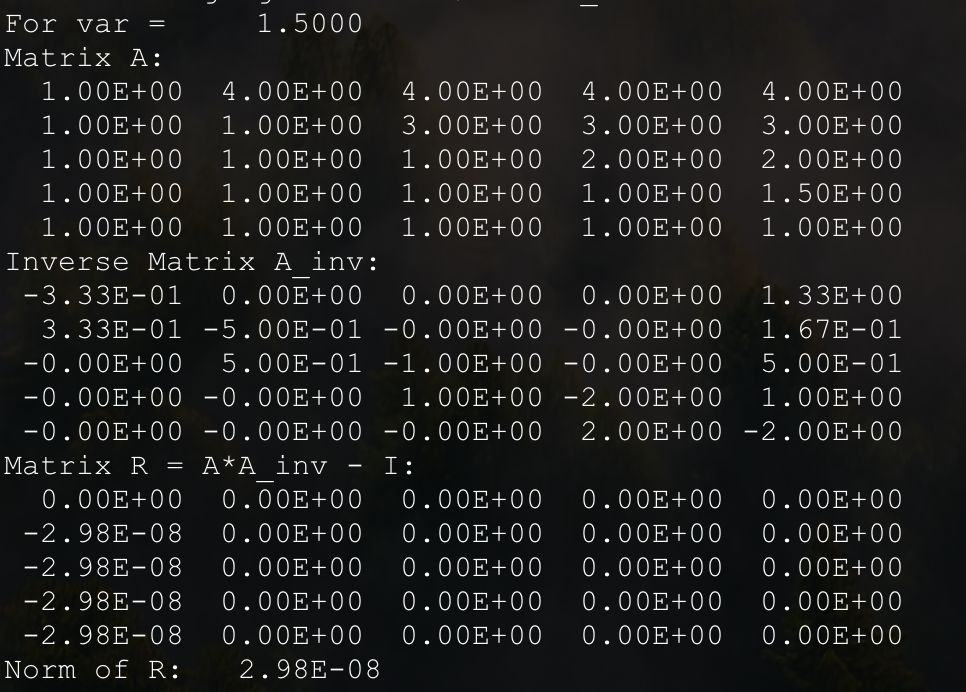
\includegraphics[width=170mm]{var_1_5.png}\\

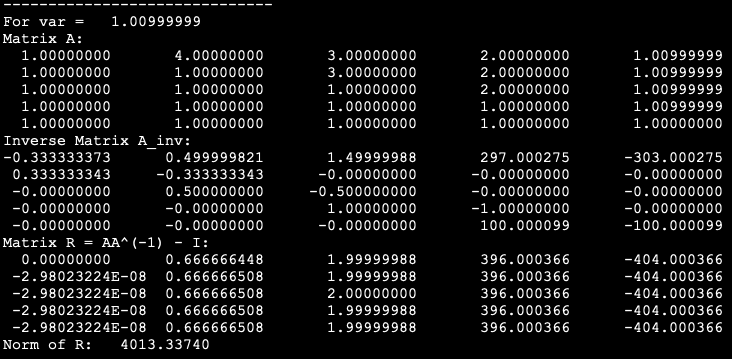
\includegraphics[width=170mm]{var_1_0.png}

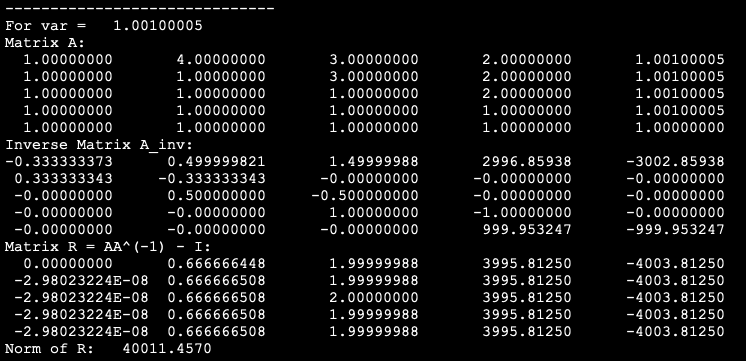
\includegraphics[width=170mm]{var_1_001.png}\\

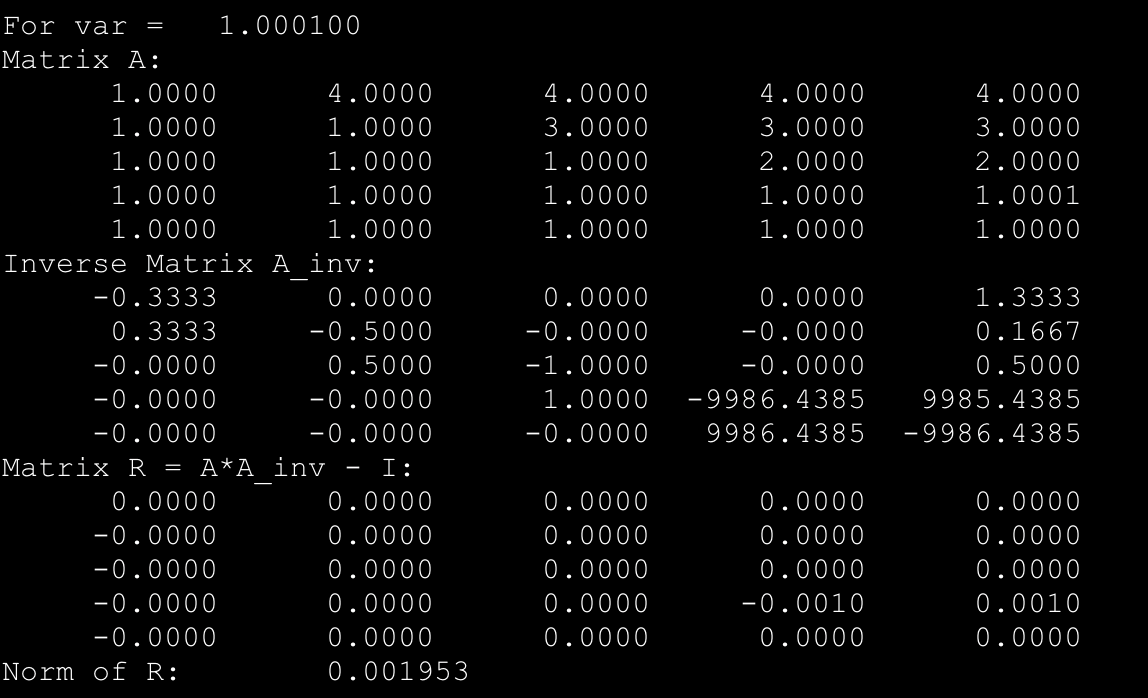
\includegraphics[width=170mm]{var_1_0001.png}

\end{document}